\documentclass[aspectratio=169]{beamer}              % only frames

% for themes, etc.
\mode<presentation>
\usetheme{Madrid} 
\usecolortheme{crane}

%\usepackage{times}  % fonts are up to you
% The usual suspects
\usepackage{multirow, booktabs, dcolumn, color, graphicx} % Tables\usepackage{graphicx}
\usepackage{amsmath,amssymb,amsthm}
% Strikethrough text
\usepackage{soul}
% Adjust box to fit tabulars
\usepackage{adjustbox}
% Embed video
\usepackage{media9}
% For notes
\usepackage{pgfpages}
%\setbeameroption{hide notes} % Only slides
%\setbeameroption{show only notes} % Only notes
\setbeameroption{hide notes} % Both
% Give a slight yellow tint to the notes page
%\setbeamertemplate{note page}{\pagecolor{yellow!5}\insertnote}\usepackage{palatino}
% Use colors by name
\usepackage{xcolor}
% EMBEDDING VIDEO IS POSSIBLE WITH PDFPC USE PDF PC to present
\usepackage{multimedia}



% The table highlighting for hypothesis discussion.
\usepackage[beamer,customcolors]{hf-tikz}
\usetikzlibrary{calc}

% To use background images
\newenvironment{colorframe}[2][]{%
\setbeamercolor{background canvas}{bg=#1}
\begin{frame}\color{white}}
{\end{frame}}


% To set the hypothesis highlighting boxes red.
\tikzset{hl/.style={
    set fill color=red!80!black!40,
    set border color=red!80!black,
  },
}

% Set Graphics folder
\graphicspath{{./figures/}}


% these will be used later in the title page
\title{Computer Networks}
\subtitle{What is the Internet?}
\author{Irfan Kanat}
\institute[CBS]{{Department of Digitization}\\ Copenhagen Business School}
\date{\today}



\begin{document}

% this prints title, author etc. info from above
\begin{frame}

	\titlepage

\end{frame}

\note{We will talk about what the internet is and why it is such a lawless territory.

We will learn about what it takes to send and receive packages across networks.}

\begin{frame}
	\frametitle{Internet is not Some Magical Mystery Land}

	\centering

	\includegraphics<1>[width = \textwidth, height = .85\textheight, keepaspectratio]{figures/ISPTiers.png}
    \includegraphics<2>[width = \textwidth, height = .85\textheight, keepaspectratio]{figures/UnderWater.png}

\end{frame}

\note{Most people imagine internet as this magical mystery land that just works. 

In reality it is a bunch of routers connected to each other.

Then who owns these routers we trust with our network traffic?

Our network traffic goes over network equipment not owned by us. This has security implications.

This is why we encrypt our traffic whenever we can.

\vfill {\tiny Image by Ludovic.ferre / CC BY-SA }}



\begin{frame}
	\frametitle{Routing The Rough Idea}

	% The internet is not some magical mysteryland
	% it is actually (SUPRISE) a network of networs
	% So when you click the link "Super cute cat AWWW :heart: :heart:"
	% Your browser creates a request, hands it to IP protocol. 
	% Your computer packs the request neatly and forwards it to your router
	% Your router replaces the IP and MAC layers and forwards it further
	% The MAC address keeps changing with each hop, but your public IP remains the same

	% At the end you get Grumpy cat on your laptop. 
	% You are happy
	% I am happy
	% everyone except grumpy cat is happy

	\only<1>{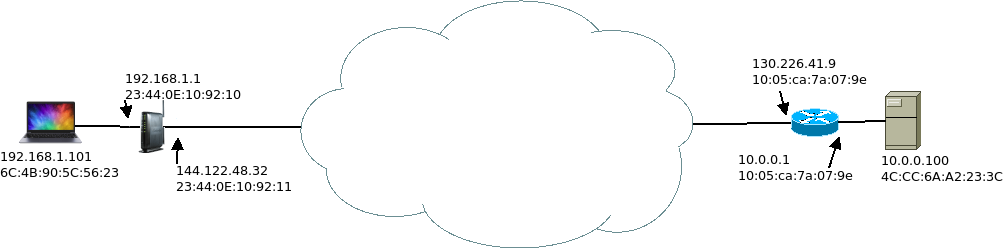
\includegraphics[width = \textwidth, height = .85\textheight, keepaspectratio]{figures/RoutingA.png} }    
	\only<2>{\movie{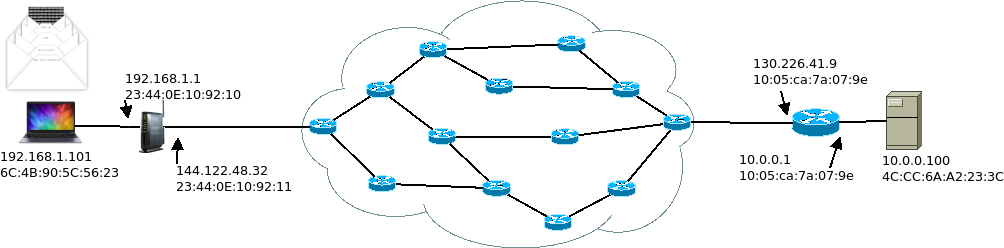
\includegraphics[width = \textwidth, height = .85\textheight, keepaspectratio]{figures/Routing020.png}}{figures/Routing.mp4}}


\end{frame}


\note{
	The internet is not some magical mysteryland
	
	It is actually (SUPRISE) a network of networks
	
	So when you click the link "Super cute cat AWWW :heart: :heart:"
	
	Your browser creates a request, hands it to TCP/IP socket. 
	
	Your computer packs the request neatly and forwards it to your router.
	
	Your router replaces the MAC addresses and forwards it further.
	
	The MAC address keeps changing with each hop, but IPs remain the same.

	At the end you get Grumpy cat on your laptop. 
	
	You are happy, I am happy, everyone except grumpy cat is happy}


\begin{frame}
	\frametitle{Big Question}

	How is the path determined? \vspace{1em}

	What constitutes the path? \vspace{1em}

	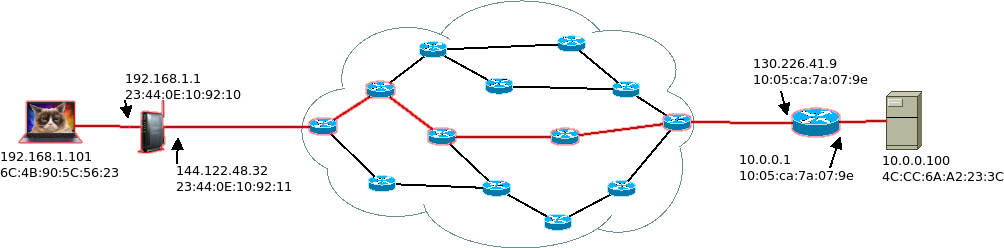
\includegraphics[width = \textwidth, height = .85\textheight, keepaspectratio]{figures/RoutingPath.png} 

\end{frame}


\begin{frame}
\frametitle{Components}

	\begin{columns}
		\begin{column}{0.5\textwidth}

			L2 Switch \vspace{1em}

			L3 Router \vspace{1em}

			Lines are blurred
	
		\end{column}

		\begin{column}{0.5\textwidth}

			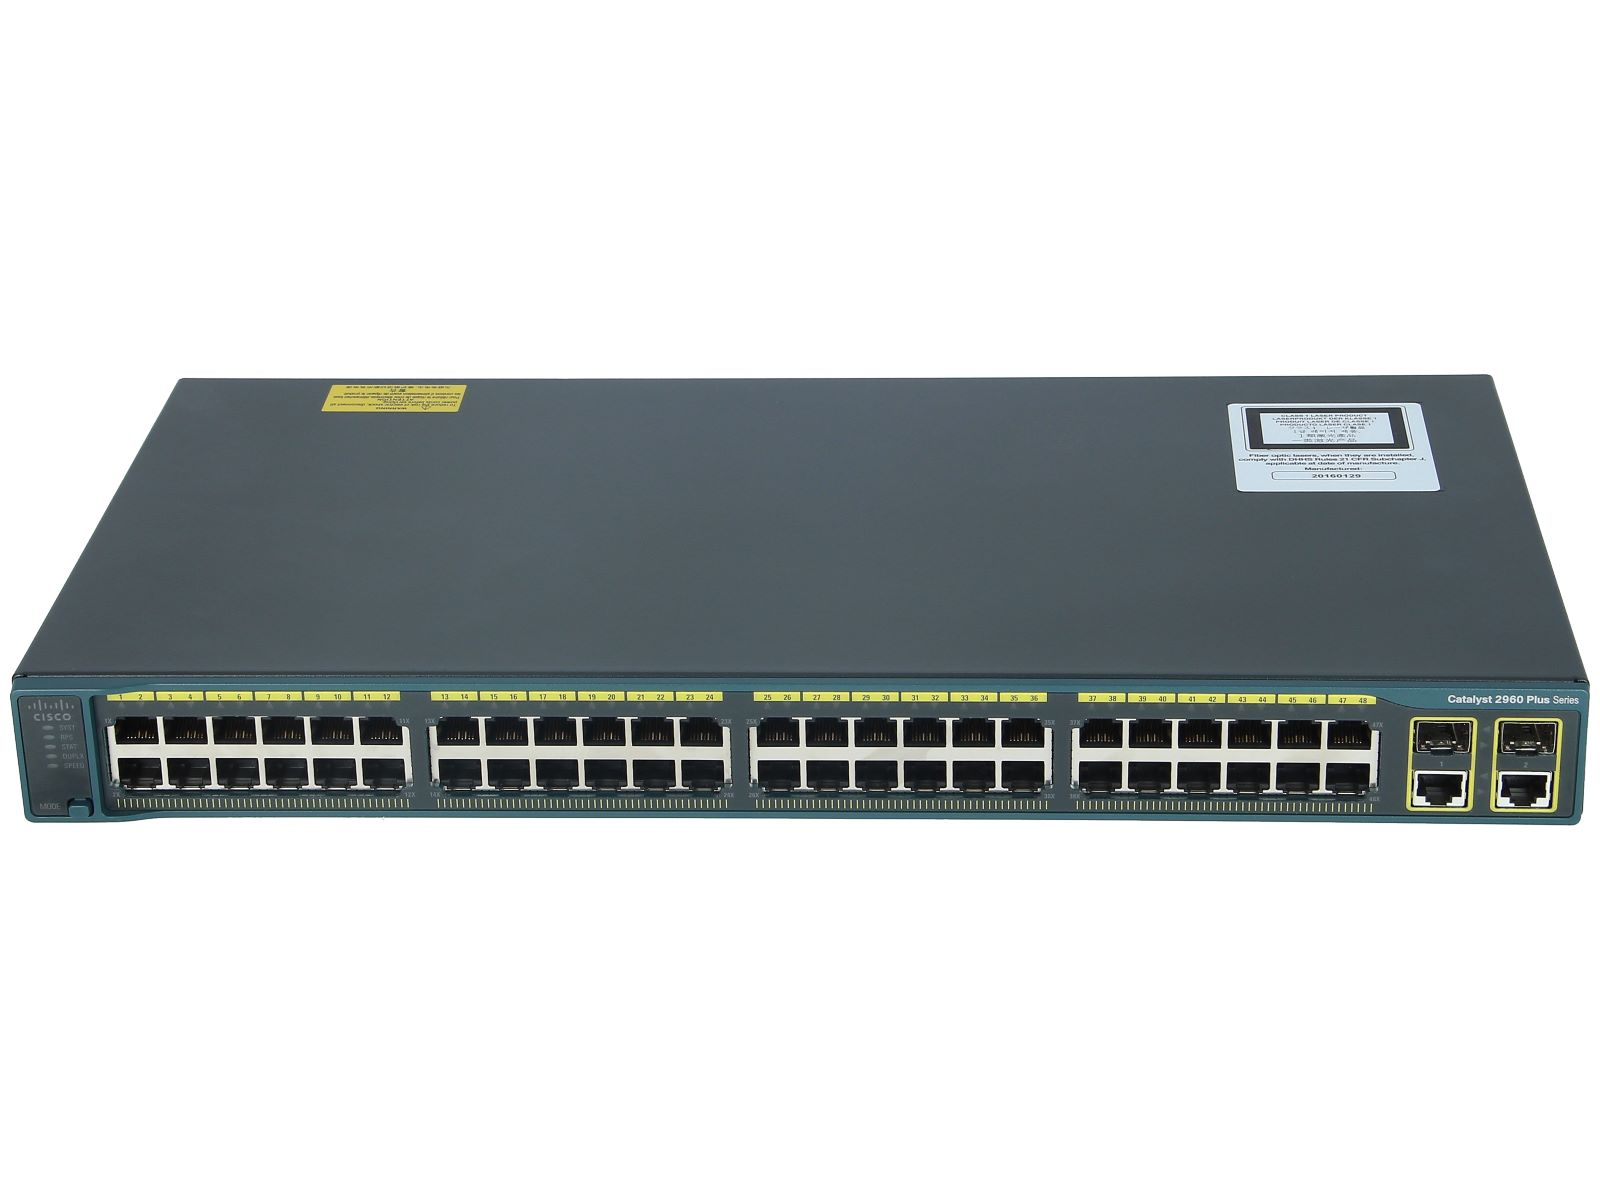
\includegraphics[width = \textwidth, height = .85\textheight, keepaspectratio]{figures/switch.jpg}

		\end{column}

	\end{columns}

\end{frame}


\begin{frame}
	\frametitle{Routing: Hardware and Layers}

	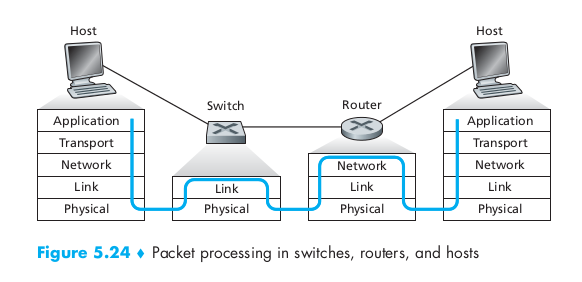
\includegraphics[width = \textwidth, height = .85\textheight, keepaspectratio]{figures/RoutingLayers.png}  

\end{frame}


\begin{frame}
\frametitle{How a Switch Works}

	\only<1>{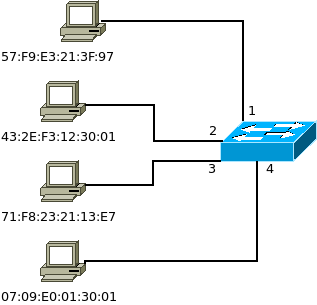
\includegraphics[width = \textwidth, height = .85\textheight, keepaspectratio]{figures/SwitchOperation1.png}}
	\only<2>{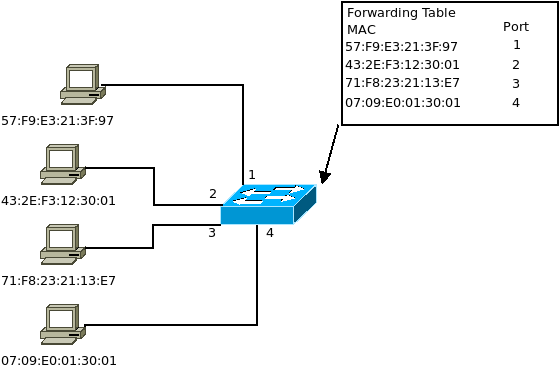
\includegraphics[width = \textwidth, height = .85\textheight, keepaspectratio]{figures/SwitchOperation2.png}}

\end{frame}

\note{
	In traditional sense a Switch operates at L2 (Datalink Layer).

	That means Switches deal with MAC addresses.

	Switches are self learning.

	They start with an empty forwarding table.

	It learns by:
		\begin{enumerate}
			\item Reading the source MAC address of incoming frame
			\item Reading the destination MAC, if not found broad cast to all ports
			\item Once a destination computer responds, its MAC address will also be associated with a port
		\end{enumerate}

	Nowadays it is also common to find L3 switches that are like routers as well.
}



\begin{frame}
	\frametitle{Brief Reminder: IP Addressing}

    \begin{columns}
		\begin{column}{0.5\textwidth}

			IP address \vspace{1em}

			\textcolor{orange}{Prefix:} A Network 

		    \textcolor{red}{Suffix:} A Node \vspace{1em}

		    \colorbox{orange}{144.122.98.}\colorbox{red}{32}
	
		\end{column}

		\begin{column}{0.5\textwidth}

			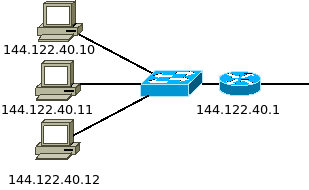
\includegraphics[width = \textwidth, height = .85\textheight, keepaspectratio]{figures/2LANsIPHalf.png}

		\end{column}

	\end{columns}

\end{frame}


\note{
	IP addresses indicate both the network and the specific node in a network.

	IP addresses are 32 binary bits. Usually first so many bits specify the network prefix.

	For the sake of simplicity I am not going into details such as subnet masks. 

	Just know that IP address allow you to identify a network (through prefix) and a node in that network (suffix)

}


\begin{frame}
	\frametitle{How a Router Works}
    
    \only<1>{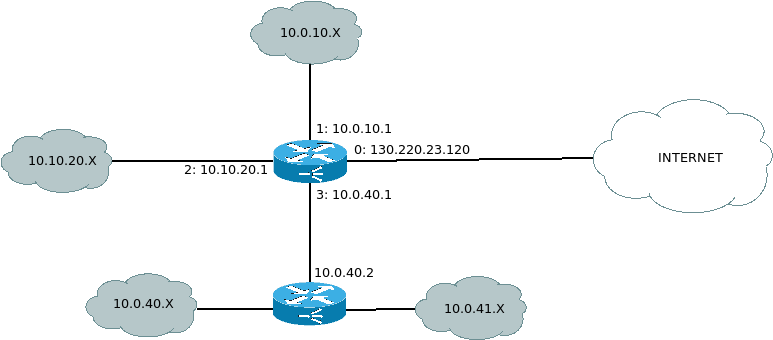
\includegraphics[width = \textwidth, height = .85\textheight, keepaspectratio]{RouterInterfaceIPs.png}}
    \only<2>{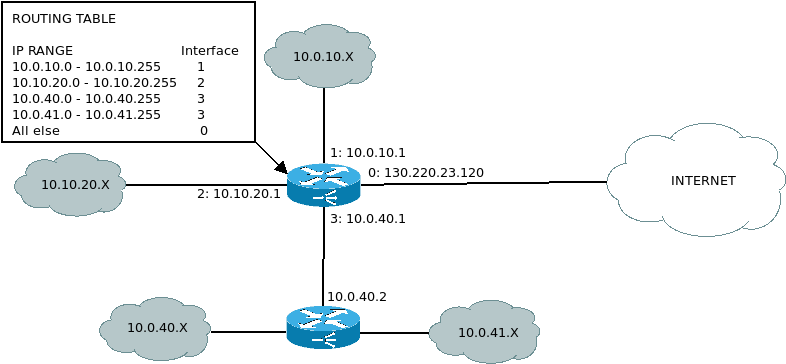
\includegraphics[width = \textwidth, height = .85\textheight, keepaspectratio]{RouterInterfaceIPs2.png} }

\end{frame}

\note{
	A router connects different networks.

	Router operates at L3 (Network Layer), so it deals with IP addresses.

	Each interface the router has with the network gets an IP address that belongs in that network.

	So the router appears to be part of multiple networks.
}

{
\usebackgroundtemplate{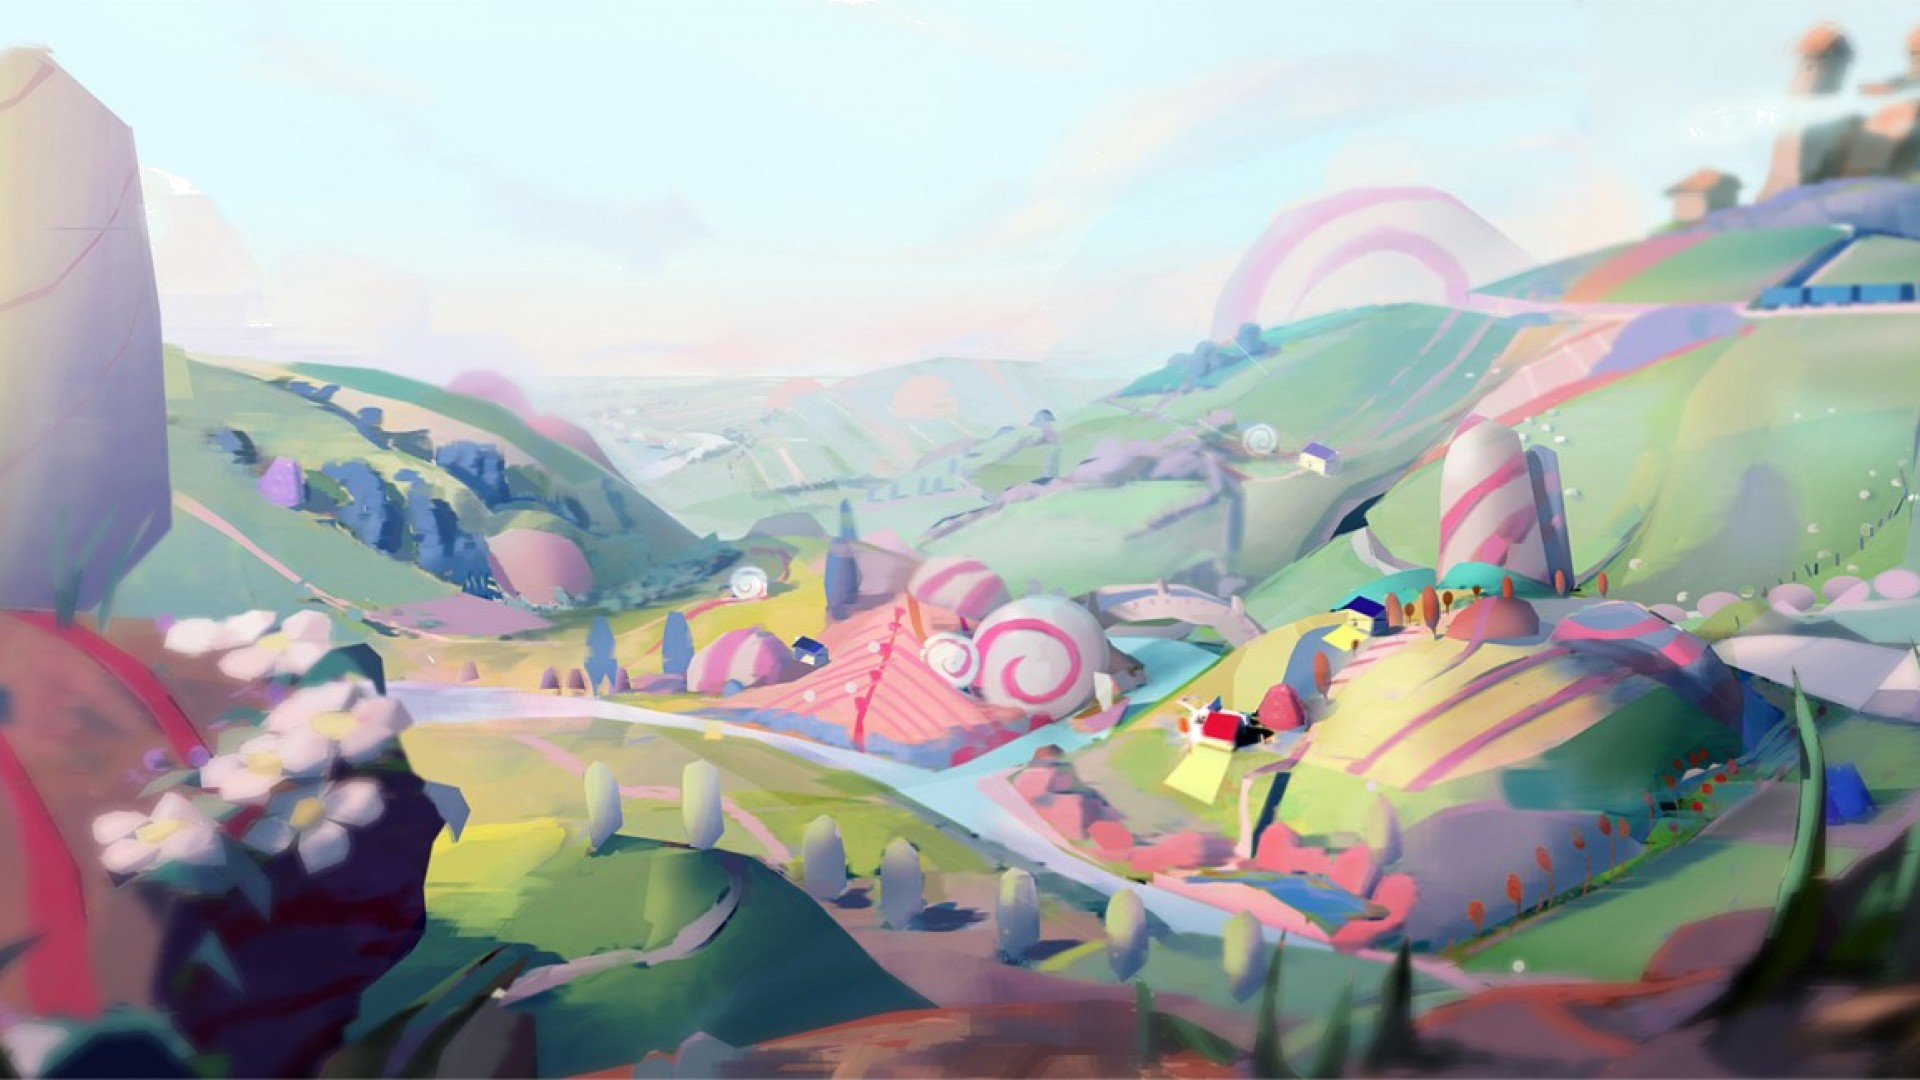
\includegraphics[width=\paperwidth,height=\paperheight]{demoland.png}}%
	\begin{frame}
	\frametitle{Forwarding in Layer 2 and Layer 3}



	\end{frame}
}

\note{Our computers more or less do the same thing as the devices discussed. Of course the number of interfaces are very limited.

For the layer 2

	arp

For the layer 3

	ip route

}


\begin{frame}
	\frametitle{Next Hop Forwarding}
	
	\only<1>{To send from A to G
	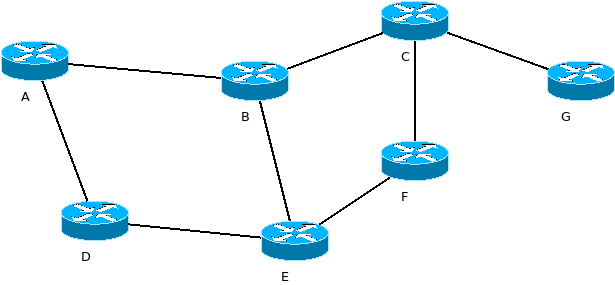
\includegraphics[width = \textwidth, height = .85\textheight, keepaspectratio]{figures/RoutingExample0.png} }
	\only<2>{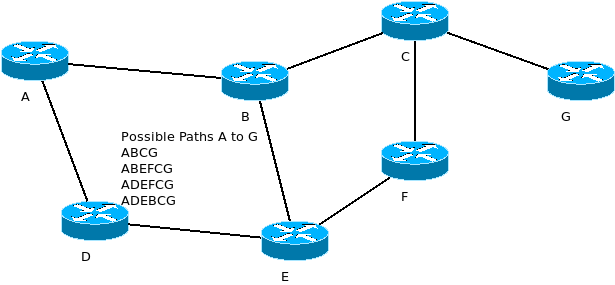
\includegraphics[width = \textwidth, height = .85\textheight, keepaspectratio]{figures/RoutingExample1.png} }
	\only<3>{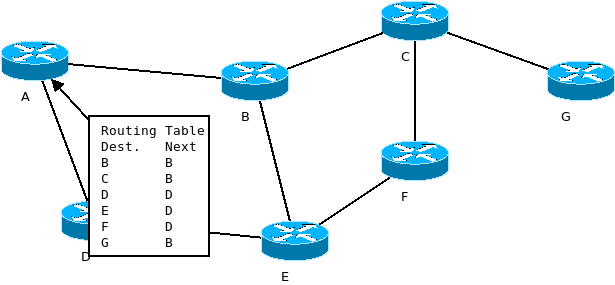
\includegraphics[width = \textwidth, height = .85\textheight, keepaspectratio]{figures/RoutingExample2.png} }
	\only<4>{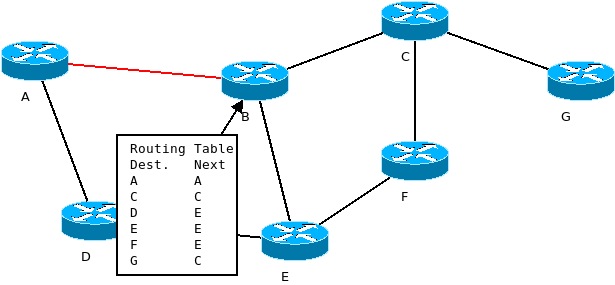
\includegraphics[width = \textwidth, height = .85\textheight, keepaspectratio]{figures/RoutingExample3.png} }
	\only<5>{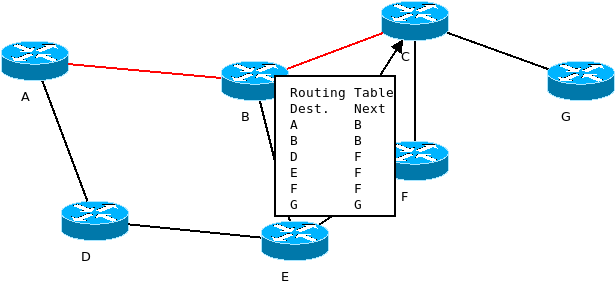
\includegraphics[width = \textwidth, height = .85\textheight, keepaspectratio]{figures/RoutingExample4.png} }
	\only<6>{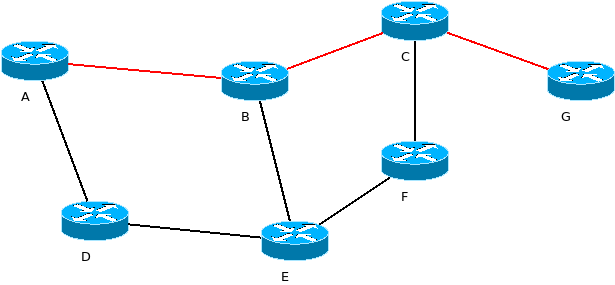
\includegraphics[width = \textwidth, height = .85\textheight, keepaspectratio]{figures/RoutingExample5.png} }
	
\end{frame}


\note{
	What routers do is called \emph{Next Hop Forwarding}.

	They only send the package to the next router along the way. 

	They figure out where to send the packages by referring to a Routing Table.

	Routing table is essentially a list of networks and associated interfaces for the router.

	The next hop forwarding does not need complete information of the network. (Otherwise every router would have to map the whole of internet.)
}

{
\usebackgroundtemplate{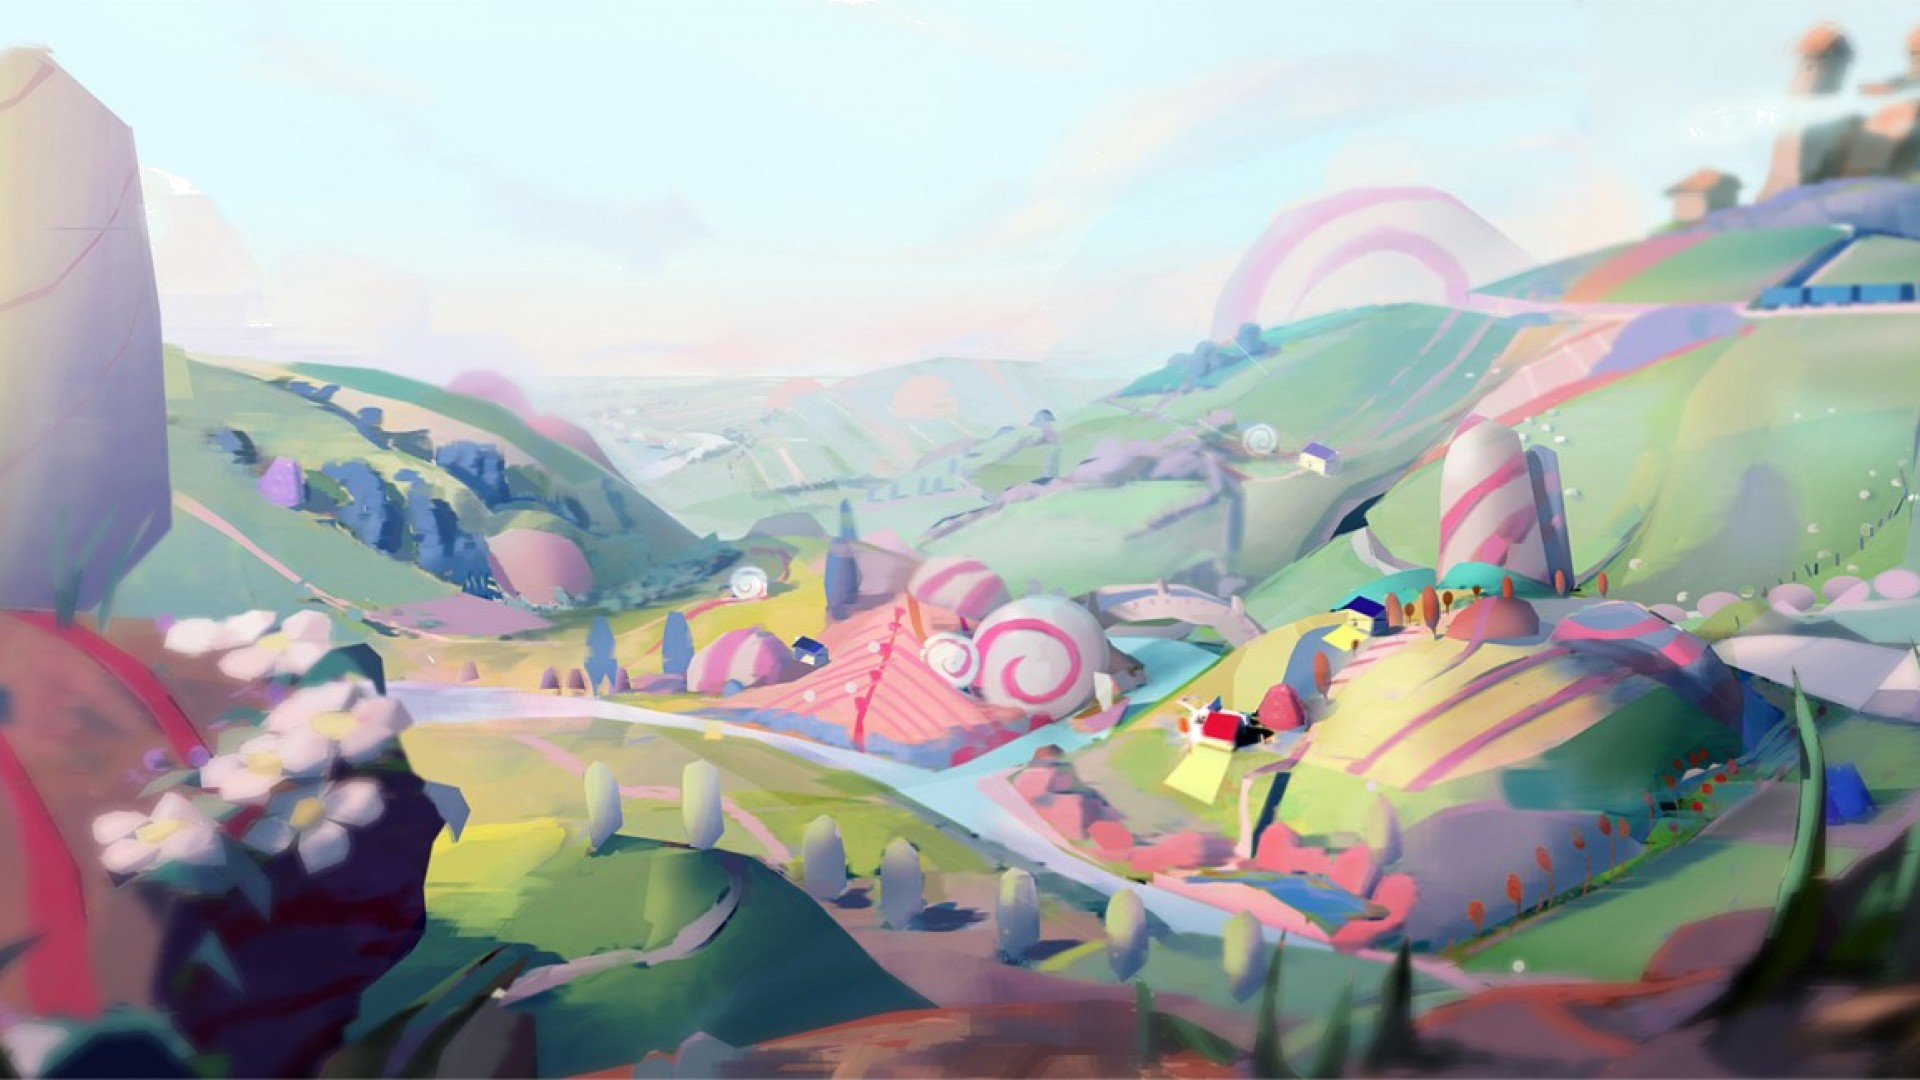
\includegraphics[width=\paperwidth,height=\paperheight]{demoland.png}}%
	\begin{frame}
	\frametitle{Trace Route}



	\end{frame}
}


\begin{frame}
	\frametitle{Populating Routing Tables: Routing Algorithms}

	Consider the size of the Internet. \vspace{1em}

	How would you populate the Routing Tables. \vspace{1em}

	\only<2>{
	\begin{itemize}
		\item Internal Routing (OSPF, RIP)
		\item External Routing (BGP)\vspace{1em}
	\end{itemize}
	}

	\only<3>{
	Considerations:
	\begin{itemize}
		\item Number of Hops
		\item Congestion
		\item Speed of circuit
	\end{itemize}
	}

\end{frame}

\note{What is interesting is that this whole process is (with some exceptions) decentralized and distributed. 

Routers exchange messages as to the availability of reachable networks and the conditions. 

Then each node decides on how to shape their own routing table with this information.
}




\end{document}
